% Actor (policy) network of the MAPPO coverage agent, see src/models/actor_critic.py.
% Compile standalone:  pdflatex policy_network.tex
% Include in a paper:  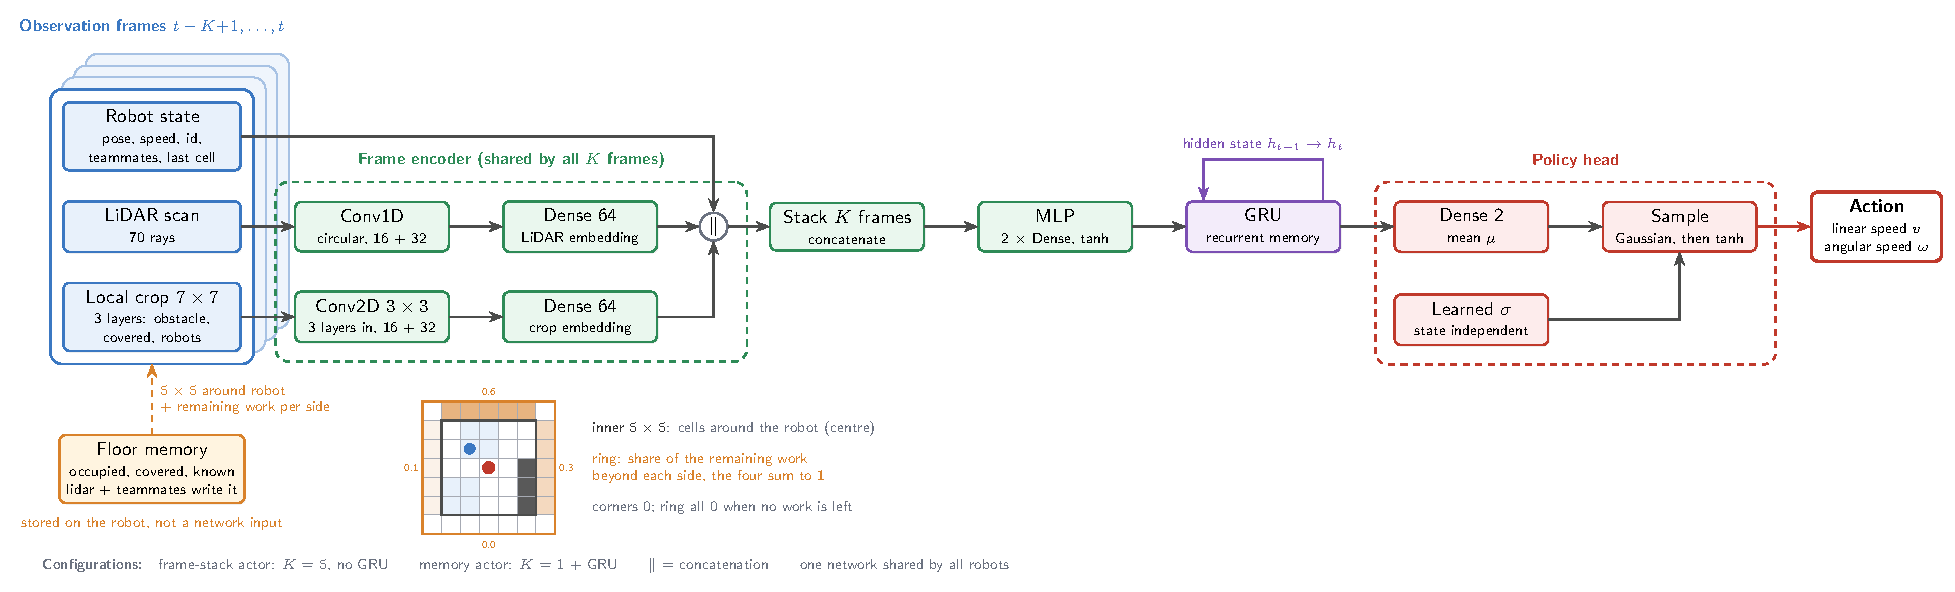
\includegraphics{policy_network.pdf}
\documentclass[tikz,border=6pt]{standalone}
\usepackage[T1]{fontenc}
\usepackage{lmodern}
\usetikzlibrary{positioning,fit,backgrounds,arrows.meta,calc,shadows}

% Palette
\definecolor{cIn}{HTML}{E8F1FB}    \definecolor{cInD}{HTML}{3B78C2}
\definecolor{cEnc}{HTML}{EAF7EE}   \definecolor{cEncD}{HTML}{2E8B57}
\definecolor{cMap}{HTML}{FFF4E0}   \definecolor{cMapD}{HTML}{D9822B}
\definecolor{cMem}{HTML}{F3ECFA}   \definecolor{cMemD}{HTML}{7B4FB3}
\definecolor{cOut}{HTML}{FDECEC}   \definecolor{cOutD}{HTML}{C0392B}
\definecolor{cGrey}{HTML}{6B7280}

\tikzset{
  font=\sffamily\small,
  >={Stealth[length=2.2mm]},
  block/.style={draw=#1D, fill=#1, rounded corners=3pt, line width=0.7pt,
                minimum height=8mm, minimum width=26mm, align=center,
                drop shadow={opacity=0.12, shadow xshift=0.6pt, shadow yshift=-0.6pt}},
  inp/.style={block=cIn, minimum width=30mm},
  enc/.style={block=cEnc},
  mapb/.style={block=cMap},
  memb/.style={block=cMem},
  head/.style={block=cOut},
  op/.style={circle, draw=cGrey, fill=white, line width=0.7pt, inner sep=1.2pt,
             font=\sffamily\bfseries\small},
  group/.style={draw=#1, dashed, rounded corners=6pt, line width=0.8pt, inner sep=9pt},
  title/.style={font=\sffamily\bfseries\footnotesize, text=#1},
  note/.style={font=\sffamily\scriptsize, text=cGrey, align=center},
  flow/.style={->, line width=0.8pt, draw=black!70},
}

\begin{document}
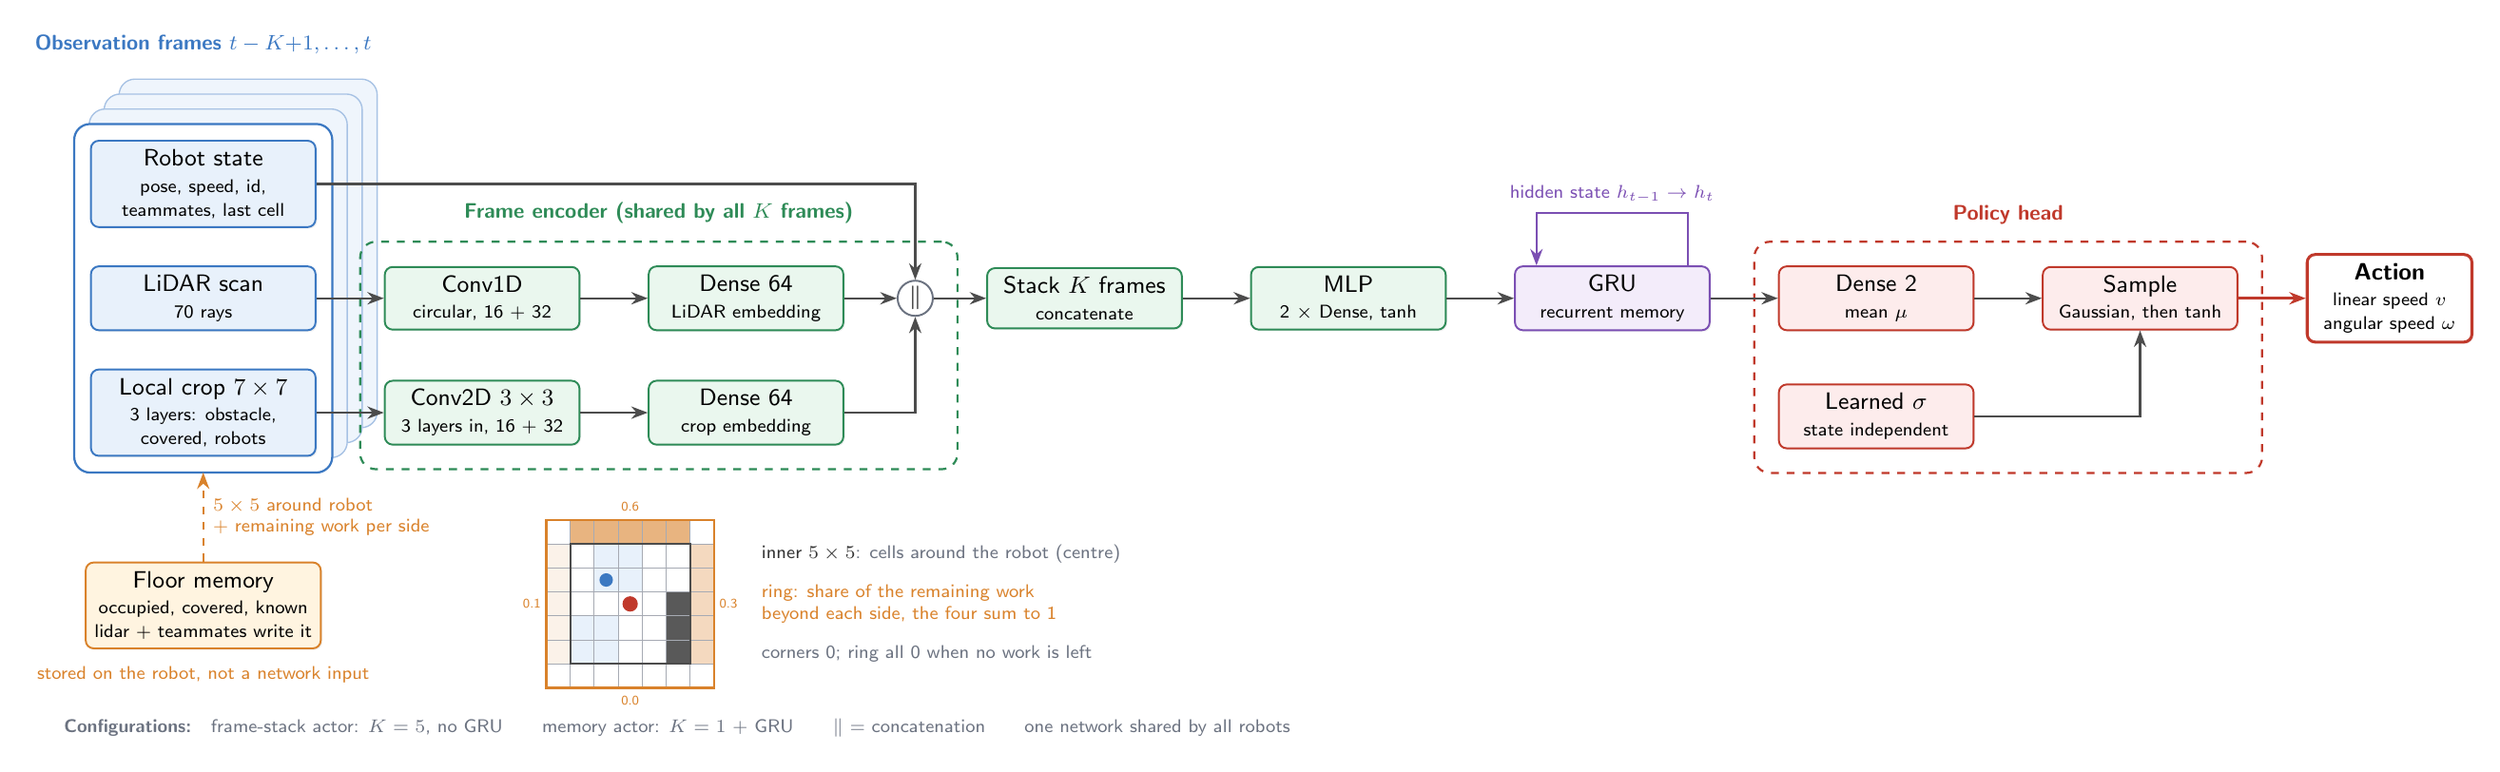
\begin{tikzpicture}[node distance=5mm and 9mm]

% ------------------------------------------------------------------ inputs
\node[inp] (vec)   {Robot state\\[-1pt]\scriptsize pose, speed, id,\\[-2pt]\scriptsize teammates, last cell};
\node[inp, below=of vec]   (lidar) {LiDAR scan\\[-1pt]\scriptsize 70 rays};
\node[inp, below=of lidar] (crop)  {Local crop $7\times7$\\[-1pt]\scriptsize 3 layers: obstacle,\\[-2pt]\scriptsize covered, robots};

% stacked-frame look behind the three per-frame inputs
\begin{scope}[on background layer]
  \foreach \s in {3,2,1}
    \node[draw=cInD!45, fill=cIn!70, rounded corners=6pt, line width=0.5pt,
          fit=(vec)(lidar)(crop), inner sep=6pt,
          xshift=\s*2mm, yshift=\s*2mm] {};
  \node[draw=cInD, fill=white, rounded corners=6pt, line width=0.8pt,
        fit=(vec)(lidar)(crop), inner sep=6pt] (frames) {};
\end{scope}
\node[title=cInD, above=8mm of frames.north] {Observation frames $t-K{+}1,\dots,t$};

% the floor memory lives on the robot: it is not a network input, it only
% supplies the local crop
\node[mapb, below=14mm of crop, minimum width=30mm] (pmap)
  {Floor memory\\[-1pt]\scriptsize occupied, covered, known\\[-2pt]\scriptsize lidar + teammates write it};
\draw[flow, dashed, draw=cMapD] (pmap.north) -- node[note, right, text=cMapD, align=left]
  {$5\times5$ around robot\\ + remaining work per side}
  ($(crop.south)+(0,-6pt)$);
\node[note, below=1mm of pmap, text=cMapD] {stored on the robot, not a network input};

% the 7x7 crop: 5x5 cells around the robot inside a one-cell directional ring.
% Example shares of the remaining work: N 0.6, E 0.3, W 0.1, S 0 (sum 1).
\begin{scope}[shift={($(pmap.east)+(30mm,-11mm)$)}, x=3.2mm, y=3.2mm]
  \fill[cMapD, opacity=0.60] (1,6) rectangle (6,7);    % north
  \fill[cMapD, opacity=0.30] (6,1) rectangle (7,6);    % east
  \fill[cMapD, opacity=0.10] (0,1) rectangle (1,6);    % west
  \fill[cIn] (2,4) rectangle (4,6);  \fill[cIn] (1,1) rectangle (3,3);   % covered cells
  \fill[black!65] (5,1) rectangle (6,4);                              % an obstacle
  \draw[cGrey!60, line width=0.3pt] (0,0) grid[step=1] (7,7);
  \draw[cMapD, line width=0.8pt] (0,0) rectangle (7,7);
  \draw[black!70, line width=0.8pt] (1,1) rectangle (6,6);
  \fill[cOutD] (3.5,3.5) circle (0.32);                                % this robot
  \fill[cInD] (2.5,4.5) circle (0.28);                                 % a teammate
  \foreach \v/\x/\y in {0.6/3.5/7.55, 0.0/3.5/-0.55, 0.3/7.6/3.5, 0.1/-0.6/3.5}
    \node[font=\sffamily\tiny, text=cMapD] at (\x,\y) {\v};
  \node[note, anchor=west, align=left] at (8.6,5.6) {\textcolor{black!80}{inner $5\times5$}: cells around the robot (centre)};
  \node[note, anchor=west, align=left, text=cMapD] at (8.6,3.5) {ring: share of the remaining work\\beyond each side, the four sum to 1};
  \node[note, anchor=west, align=left] at (8.6,1.4) {corners 0; ring all 0 when no work is left};
\end{scope}

% ------------------------------------------------------------------ frame encoder
\node[enc, right=of lidar] (conv1) {Conv1D\\[-1pt]\scriptsize circular, 16 + 32};
\node[enc, right=of conv1] (lemb)  {Dense 64\\[-1pt]\scriptsize LiDAR embedding};
\node[op,  right=7mm of lemb] (cat1) {$\Vert$};
\draw[flow] (lidar) -- (conv1);
\draw[flow] (conv1) -- (lemb);
\draw[flow] (lemb) -- (cat1);
\node[enc, right=of crop]  (conv2) {Conv2D $3\times3$\\[-1pt]\scriptsize 3 layers in, 16 + 32};
\node[enc, right=of conv2] (cemb)  {Dense 64\\[-1pt]\scriptsize crop embedding};
\draw[flow] (crop) -- (conv2);
\draw[flow] (conv2) -- (cemb);
\draw[flow] (vec.east)  -| (cat1.north);
\draw[flow] (cemb.east) -| (cat1.south);

\node[enc, right=7mm of cat1] (stack) {Stack $K$ frames\\[-1pt]\scriptsize concatenate};
\draw[flow] (cat1) -- (stack);

\begin{scope}[on background layer]
  \node[group=cEncD, fit=(conv1)(lemb)(cat1)(conv2)(cemb)] (encbox) {};
\end{scope}
\node[title=cEncD, above=1mm of encbox.north] {Frame encoder (shared by all $K$ frames)};

% ------------------------------------------------------------------ trunk + GRU
\node[enc, right=of stack] (mlp) {MLP\\[-1pt]\scriptsize 2 $\times$ Dense, tanh};
\node[memb, right=of mlp] (gru) {GRU\\[-1pt]\scriptsize recurrent memory};
\draw[flow] (stack) -- (mlp);
\draw[flow] (mlp) -- (gru);

% recurrent loop
\draw[flow, draw=cMemD] (gru.north east) ++(-3mm,0) -- ++(0,7mm) -| node[note, pos=0.25, above, text=cMemD] {hidden state $h_{t-1}\rightarrow h_t$} ($(gru.north west)+(3mm,0)$);

% ------------------------------------------------------------------ head
\node[head, right=of gru] (mu) {Dense 2\\[-1pt]\scriptsize mean $\mu$};
\node[head, below=7mm of mu] (sigma) {Learned $\sigma$\\[-1pt]\scriptsize state independent};
\node[head, right=of mu] (sample) {Sample\\[-1pt]\scriptsize Gaussian, then tanh};
\draw[flow] (gru) -- (mu);
\draw[flow] (mu) -- (sample);
\draw[flow] (sigma.east) -| (sample.south);

\node[head, fill=white, draw=cOutD, line width=1.1pt, right=of sample, minimum width=22mm] (act)
  {\textbf{Action}\\[-1pt]\scriptsize linear speed $v$\\[-2pt]\scriptsize angular speed $\omega$};
\draw[flow, line width=1.1pt, draw=cOutD] (sample) -- (act);

\begin{scope}[on background layer]
  \node[group=cOutD, fit=(mu)(sigma)(sample)] (headbox) {};
\end{scope}
\node[title=cOutD, above=1mm of headbox.north] {Policy head};

% ------------------------------------------------------------------ legend
\node[note, align=left, anchor=north west] at ($(pmap.south west)+(-4mm,-8mm)$)
  {\textbf{Configurations:}\quad
   frame-stack actor: $K=5$, no GRU\qquad
   memory actor: $K=1$ + GRU\qquad
   $\Vert$ = concatenation\qquad
   one network shared by all robots};

\end{tikzpicture}
\end{document}
